\documentclass[../src/handouts/main.tex]{subfiles}
% note that the CWD (.) above is the output directory of pdflatex
% (<repo-root-dir>/build)

% path that contains required images
\graphicspath{ {../src/handouts/figures/} }

% This document depends on introduction.tex, which provides
% fig:intro-special-functions, def:intro-equiv-relation.
% As a result, compiling only this document gives undefined references.

% prevent \recall theorems outside this section
% if this section is compiled solely
\def\sectionprefix{con}%

\begin{document}

\section{Fundamental Concepts}

% argument can be: empty or any string. Any non empty string will produce a graph with labels (people, jobs)
% ref: https://stackoverflow.com/a/2145370
\newcommand\bipartitegraphhelper[1]{
  \begin{tikzpicture}[
      point/.style = {circle, fill=black, inner sep=1mm}]
    \def \distance {1.5} %
    \foreach \x in {0,...,3} % 0 = leftmost; 3 = rightmost
    \foreach \y in {0,...,1} % 0 = top row; 1 = bottom row
    \node[point] (\y\x) at (\x * \distance, \y * - \distance) {};

    \draw (00) -- (10) -- (01) -- (11) -- (03) -- (10);
    \draw (12) -- (02) -- (13);

    % ref: https://tex.stackexchange.com/a/195498
    \ifthenelse{\isempty{#1}}%
    {}%
    {
      \node at (4 * \distance, 0) {people}
      node at (4 * \distance, - \distance) {jobs};
    }%
  \end{tikzpicture}
}%

\def \bipartitegraph{\bipartitegraphhelper{}}%

\def \bipartitegraphwithlabels {\bipartitegraphhelper{with labels}}%

\def \tripartitegraph {%
  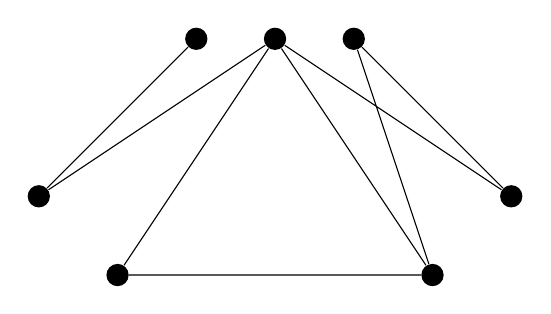
\begin{tikzpicture}[every node/.style = {circle, fill=black, inner sep=1mm}]
    \node (a1) at (-3, 1) {} % left, top
    node (a2) at (-2, 0) {} % left, bottom
    node (b1) at (-1, 3) {} % top, left
    node (b2) at (0, 3) {} % top, middle
    node (b3) at (1, 3) {} % top, right
    node (c1) at (2, 0) {} % right, bottom
    node (c2) at (3, 1) {}; % right, top
    \draw (b1) -- (a1) -- (b2) -- (a2) -- (c1) -- (b2) -- (c2) -- (b3) -- (c1);
  \end{tikzpicture}
}%

This section is the chapter one in the textbook "Introduction to Graph Theory". It covers all key concepts, keywords, definitions, theorems, etc.

\subsection{Graph}

\begin{definition}{}{con-graph}
  (1.1.2. Definition in text, modified version)
  A \textbf{graph} $G$ contains:
  \begin{enumerate}
    \item A \textbf{vertex set} $V(G)$
    \item An \textbf{edge set} $E(G)$
    \item A relation that associates with each two vertices (not necessarily distinct) called its \textbf{endpoints}.
  \end{enumerate}
\end{definition}

\Cref{def:con-graph} is a \textit{triple}, which means you need these three components to describe a graph, usually in the order of vertex set, edge set, and relations.

In \cref{def:con-graph}, for simple graphs, you could use a vertex set with either \textit{an edge set} or \textit{a relation for each edge} to define a graph. But for multigraphs like \cref{fig:con-graph}, in which there are multiple edges (\cref{def:con-loop}) between some two vertices, all three components of a graph are nontrivial.

An edge between vertices $u$ and $v$ can be denoted by either $\set{ u,\, v }$, $uv$ or $\left( u,\, v \right)$.

In \cref{def:con-graph}, the relation of a graph may$\ldots$
\begin{enumerate*}
  \item show the endpoints of \textit{each} edge in its edge set, or
  \item \textit{group} edges with the same endpoints and show the number of each group.
\end{enumerate*}

\begin{figure}[ht]
  \centering
  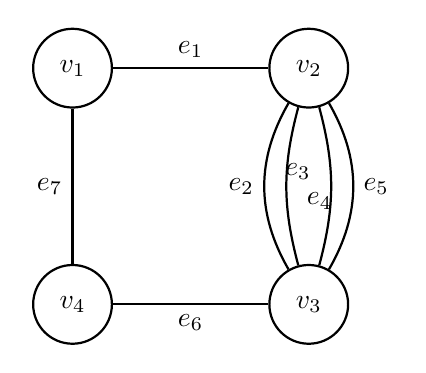
\begin{tikzpicture}[thick,
      main/.style = {draw, circle, minimum size=10mm},
      auto]
    % nodes
    \node[main] (1) at (0, 3) {$v_1$};
    \node[main] (2) at (3, 3) {$v_2$};
    \node[main] (3) at (3, 0) {$v_3$};
    \node[main] (4) at (0, 0) {$v_4$};

    % directed edges
    \draw (1) to node[above] {$e_1$} (2);
    \draw (2) to[bend right=30] node[left] {$e_2$} (3);
    \draw (2) to[bend right=15] node[right=-1.5mm, pos=.4] {$e_3$} (3);
    \draw (2) to[bend left=15] node[left=-1.5mm, pos=.6] {$e_4$} (3);
    \draw (2) to[bend left=30] node[right] {$e_5$} (3);
    \draw (3) to node[below] {$e_6$} (4);
    \draw (4) to node[left] {$e_7$} (1);
  \end{tikzpicture}
  \caption{A sample multigraph (opposite to a simple graph)}
  \label{fig:con-graph}
\end{figure}

\subsubsection{Seven Bridges of Königsberg}

Graph theory has been booming since 17th to 19th centuries.\footnote{In 1736, Leonhard Euler published a paper related to the Seven Bridges of Königsberg. This paper is regarded as the first paper in the history of graph theory, collected in \textit{Graph Theory, 1736--1936}, first published in 1976.} The initiation is the seven bridges problem in Prussia (now Russia).

In this problem, there are seven bridges among two mainlands and two islands on the Pregel river. The goal is to find a path to traverse all bridges exactly once and back to the starting point. See \cref{subsec:con-path} for more info about a path.

We have a graph as follows, shown in \cref{fig:con-seven-bridge}.
% ref: https://stackoverflow.com/a/33801400
\begin{equation*}
  G =
  \left(
  \begin{array}{l}
    \{ w,\, x,\, y,\, z \},                        \\
    \{ \foreach \i in {1,...,6} {e_\i,\, } e_7 \}, \\
    \{ wx,\, wx,\, wz,\, wz,\, wy,\, xy,\, yz \}
  \end{array}
  \right)
\end{equation*}

\begin{figure}[ht]
  \centering
  \begin{subfigure}{0.35\textwidth}
    \centering
    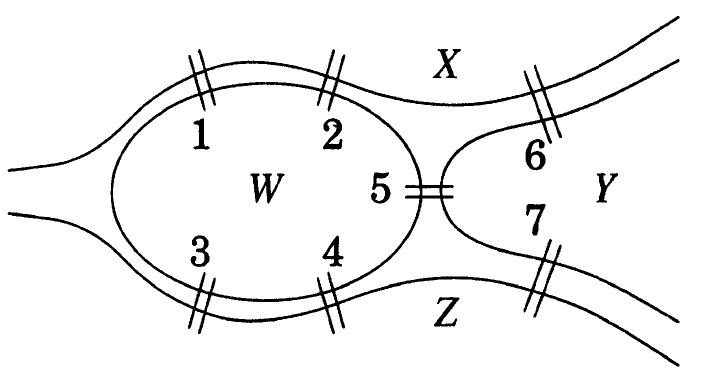
\includegraphics[width=\textwidth]{con-seven-bridge-original}
    \caption{Original version.}
    \label{fig:con-seven-bridge-original}
  \end{subfigure}
  \hspace{.1\textwidth}
  \begin{subfigure}{0.25\textwidth}
    \centering
    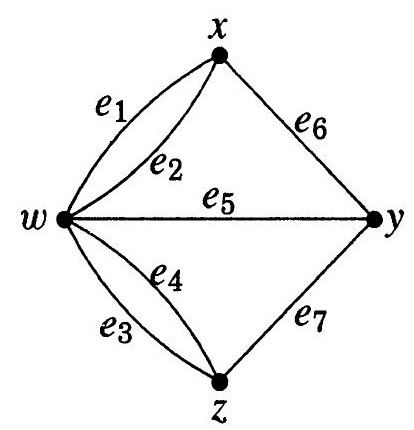
\includegraphics[width=\textwidth]{con-seven-bridge-graph}
    \caption{Graph version.}
    \label{fig:con-seven-bridge-graph}
  \end{subfigure}
  \caption{Seven-bridge problem.}
  \label{fig:con-seven-bridge}
\end{figure}

There are three principles related to the seven-bridge problem. You could try to list them on your own in advance:
\begin{enumerate*}
  \item If the degree (the number of connected edges) of each vertex is \textbf{even}, there must be a path to traverse all edges exactly once from and to the same vertex for an arbitrary vertex.
  \item If there are exactly \textbf{two} odd-degreed vertices, saying A and B, there must be a path to traverse all edges exactly once from A to B, or from B to A.
  \item If there are more than two odd-degreed vertices, three is no path to traverse all edges exactly once.
\end{enumerate*}

In the exams, you need to show why some graphs have no feasible solution with these three principles rather than showing all possible solutions.

We will cover the proofs of these principles in later sections. % TODO: link to their proofs

\subsubsection{Graph Terminologies}

\begin{definition}{}{con-loop}
  (1.1.4. Definition in text)
  A \textbf{loop} (so-called \textbf{self-loop}) is an edge whose endpoints are equal.

  \textbf{Multiple edges} are edges having the same pair of endpoints, like edges between $v_2$ and $v_3$ in a multigraph like \cref{fig:con-graph}.

  A \textbf{simple graph} is a graph having no loops or multiple edges.

  When $u$ and $v$ are the endpoints of an edge, they are \textbf{adjacent} and are \textbf{neighbors}, written $u \leftrightarrow v$.
\end{definition}

Continuing from \cref{def:con-loop}, if we have a node without a visible edge from an to it on graph, we wouldn't say that there is a self-loop.

\begin{definition}{}{con-finite-null-graph}
  (1.1.6.* Remark and the paragraph above it in text\footnote{The asterisk symbol (*) in the textbook \textit{Introduction to Graph Theory} means optional material that is not used later and can be skipped.})
  A \textbf{finite graph} has finite vertex set and edge set.

  A \textbf{null graph} (order-zero graph) has empty vertex set, and thus has empty edge set. Sometimes a null graph refers to an empty graph.

  An \textbf{empty graph} (edgeless graph) has finite vertex set and \textbf{empty} edge set.

  As for an \textbf{infinite graph}, it is usually used in Astronomy for infinite number of planets.
\end{definition}

Notice that in most cases, unless specified, we treat a graph as a simple and finite graph. In some cases, we consider null graphs and multigraphs.

\begin{definition}{}{con-complement}
  (1.1.8. Definition in text)
  The \textbf{complement} of a \textit{simple} graph $G$ is denoted by $\bar G$, which is the simple graph with vertex set $V(G)$ and edge set $E(\bar G)$ defined by $uv \in E(\bar G) \iff uv \notin E(G)$.

  A \textbf{clique} in a graph is a set of pairwise adjacent vertices. A single vertex is also a clique. However, it is controversial for a null graph to be a clique.

  An \textbf{independent set} (stable set) in a graph is a set of pairwise nonadjacent vertices. That is,
\end{definition}

\begin{figure}[ht]
  \centering
  \begin{subfigure}[t]{.3\textwidth}
    \centering
    % TODO: TikZ version
    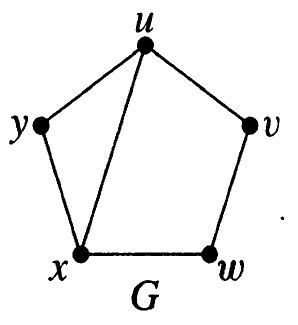
\includegraphics[width=\textwidth]{con-complement-before}
    \caption{The original graph $G$.}
    \label{fig:con-complement-before}
  \end{subfigure}
  \hspace{.1\textwidth}
  \begin{subfigure}[t]{.3\textwidth}
    \centering
    % TODO: TikZ version
    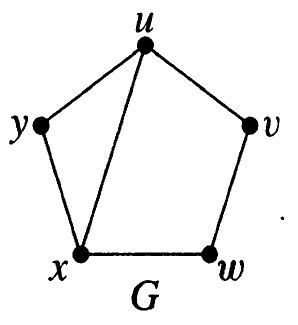
\includegraphics[width=\textwidth]{con-complement-before}
    \caption{The complement of graph $G$, denoted by $\bar G$.}
    \label{fig:con-complement-after}
  \end{subfigure}
  \caption{An example of complement of a graph. Also, vertices $u$, $x$ and $y$ in graph $G$ form a \textbf{maximal clique} of size 3 (three vertices); vertices $x$ and $w$ form a clique of size 2; vertex $u$ form a clique of size 1.}
  \label{fig:con-complement}
\end{figure}

For the complement in \cref{def:con-complement}, in brief, a complement of a graph $G$ consists of the same vertices of $G$ with all the edges \textit{not} in $G$ and without all the edges in $G$.

For the clique in \cref{def:con-complement}, note that a clique refers to a subset of vertices rather than edges or graphs.

When saying about a clique or an independent set, we usually need to find a maximal clique or a maximal independent set.

Finding a maximal clique and finding a maximal independent set are dual of each other. That is, finding a maximal clique in a graph $G$ (vertices $u,\, x,\, y$ in \cref{fig:con-complement-before}) is equal to finding an independent set in $\bar G$ (vertices $u,\, x,\, y$ in \cref{fig:con-complement-after}). \supp{If we find a maximal clique $C$ in $G$, since all vertices in $C$ are adjacent, they are all nonadjacent in $\bar G$, and it means a maximal independent set in $\bar G$.}

Finding a maximal clique, finding all cliques and finding a maximal independent set are all NP-complete problems.
And finding a maximal independent set is also a strongly NP-hard problem.

\begin{definition}{}{con-chromatic}
  (1.1.12. Definition in text)
  \textbf{Chromatic number} of a graph $G$, denoted by $\chi (G)$, is the \textit{minimum number of colors} needed to label the vertices so that adjacent vertices receive different colors.
\end{definition}

For \cref{def:con-chromatic}, that is, if two vertices has an edge between, these two vertices cannot have the same color. For a tree (because it's bipartite as shown in \cref{prop:con-bipartite-tree}), its chromatic number is 2. For a graph without edges, its chromatic number is 1.

For any finite graph (\cref{def:con-finite-null-graph}), we can find its chromatic number given that the colors can be hard for humans to distinguish (like \#FF1234 and \#FF1235 pixel values).

\supp{Chromatic numbers The complexity of finding a chromatic number is an open problem. It is likely NP-complete or NP-hard, but we couldn't find a way to reduce it to an NP-complete problem.}

\subsubsection{Bipartite Graphs}

\begin{definition}{}{con-bipartite}
  (1.1.10. Definition and 1.1.12. Definition in text)
  A graph $G$ is \textbf{bipartite} if $V(G)$ is the union of two disjoint (possibly empty) \textit{independent sets} called \textbf{bipartite sets} of $G$.

  For three disjoint independent sets, $G$ is \textbf{tripartite}.

  For $k$ disjoint independent sets, $G$ is $k$-partite (generally speaking, multipartite), where $k \in \set{ i : i \in \N \land i \geq 3}$.
\end{definition}

\begin{figure*}[ht]
  \centering
  \begin{subfigure}{.4\textwidth}
    \centering
    \bipartitegraphwithlabels
    \caption{A bipartite graph}
    \label{fig:con-bipartite}
  \end{subfigure}
  \hspace{.1\textwidth}
  \begin{subfigure}{.4\textwidth}
    \centering
    \tripartitegraph
    \caption{A tripartite graph.}
    \label{fig:con-tripartite}
  \end{subfigure}
  \caption{Bipartite and tripartite graphs.}
  \label{fig:con-bipartite-tripartite}
\end{figure*}

In \cref{fig:con-bipartite}, only people can get paid for jobs; people cannot get people (having no relation); jobs cannot get jobs. Thus, the following graph is a \textbf{bipartite graph}.

However, it is possible for all the people here to get no offers (jobs). This is a special case you need to consider in exams.

In a rooted tree like \cref{fig:con-rooted-tree}, you are able to see the children and parents of nodes, so you can find a root. In an unrooted tree like \cref{fig:con-unrooted-tree}, you couldn't. % TODO: link to tree

\begin{figure}[ht]
  \centering
  \begin{subfigure}[t]{.2\textwidth}
    \centering
    % TODO: TikZ version
    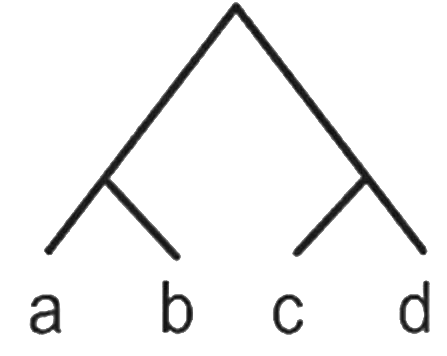
\includegraphics[width=\textwidth]{con-rooted-tree}
    \caption{A rooted tree}
    \label{fig:con-rooted-tree}
  \end{subfigure}
  \hspace{.1\textwidth}
  \begin{subfigure}[t]{.2\textwidth}
    \centering
    % TODO: TikZ version
    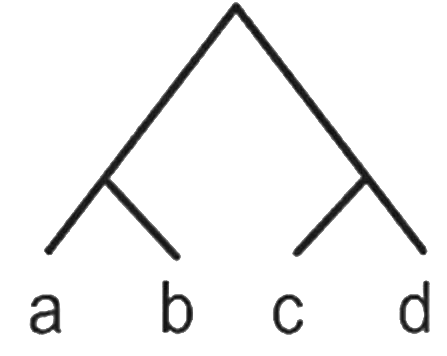
\includegraphics[width=.8\textwidth]{con-unrooted-tree}
    \caption{An unrooted tree}
    \label{fig:con-unrooted-tree}
  \end{subfigure}
  \hspace{.1\textwidth}
  \begin{subfigure}[t]{.3\textwidth}
    \centering
    % TODO: TikZ version
    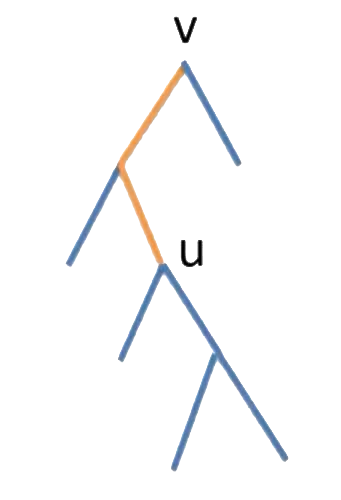
\includegraphics[width=.5\textwidth]{con-bipartite-tree}
    \caption{An illustration to prove that a rooted tree is a bipartite graph}
    \label{fig:con-bipartite-tree}
  \end{subfigure}
  \caption{Examples of rooted trees and unrooted trees}
  \label{fig:con-rooted-unrooted-trees}
\end{figure}

In programming, you could use linked lists to store a tree, but in graph theory, rooted and unrooted trees have different meaning.

\begin{proposition}{}{con-bipartite-tree}
  A tree (either rooted or unrooted one) is bipartite.
\end{proposition}

\textbf{Proof} of \cref{prop:con-bipartite-tree}:
Our goal is to find a partition of two disjoint independent sets.
Let $v$ be the root of a tree (we could pick any node, but this node is fixed in the following proof), and let $u$ be an arbitrary node in the tree.
We can find the distance between $v$ and $u$, and such a distance is a non-negative integer ($\N \cap \{ 0 \}$).
We partition all nodes in the tree into two sets: a set $S_e$ for all nodes with even distances to $v$, including $v$ itself; a set $S_o$ for all nodes with odd distances to $v$.
There is no exception for non-even and non-odd distances.
Since $S_e$ and $S_o$ are disjoint independent sets, the tree is a bipartite graph.
This applies to all trees including rooted and unrooted trees.

So, for a coloring problem on a tree, we could apply the same technique above to find two independent sets to solve the problem. We could also prove \cref{prop:con-bipartite-tree} with a coloring problem. % TODO: link to coloring problem

Note that some proofs are pretty simple, but it doesn't mean that they wouldn't be in exams.

Some comments for bipartite graphs:
\begin{enumerate}
  \item A bipartite graph is a graph with no odd length cycle. That is, there doesn't exist a path to traverse some vertices along edges and back to the starting point with odd number of edges. For a graph with no possible cycles or with only even length cycles, such a graph is also bipartite. \supp{A bonus problem is as follows. Proove that a graph is not bipartite if it has one or more \textit{arbitrary} (3, 5, 7, etc.) odd length cycles. However, in 2024 spring, announced in 2024-03-08, the bonus problem changed to a program homework with different topics.}

  \item Another ways to define an $n$-vertex tree $G$, where $n \geq 1$:
        \begin{enumerate}
          \item $G$ satisfies any two of the following three rules:
                \begin{enumerate}
                  \item $G$ is connected. (See \cref{fig:con-connected-graph-interlude} for the illustration of connected and unconnected graphs. And see \cref{def:con-connected} for the definition.)
                  \item $G$ has "$n - 1$" edges.
                  \item $G$ has no cycles. Note that a self-loop is a cycle.
                \end{enumerate}
          \item $G$ has no loops, and for each $u,\, v \in V(G)$, there exists exactly one $u,\, v$-path. (This rule is sufficient to show that $G$ is a tree, for the later part shows the three rules above.) % TODO: link to their proofs
        \end{enumerate}
\end{enumerate}

\begin{figure}[ht]
  \centering
  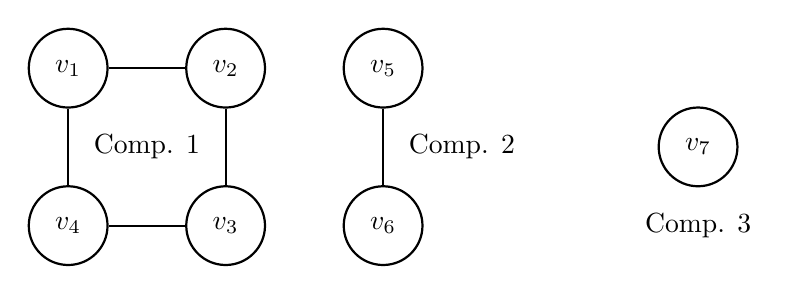
\begin{tikzpicture}[thick,
      main/.style = {draw, circle, minimum size=10mm},
      auto]
    % nodes
    \node[main] (1) at (0, 2) {$v_1$};
    \node[main] (2) at (2, 2) {$v_2$};
    \node[main] (3) at (2, 0) {$v_3$};
    \node[main] (4) at (0, 0) {$v_4$};
    \node at (1, 1) {Comp. 1};

    \node[main] (5) at (4, 2) {$v_5$};
    \node[main] (6) at (4, 0) {$v_6$};
    \node at (5, 1) {Comp. 2};

    \node[main] (7) at (8, 1) {$v_7$};
    \node at (8, 0) {Comp. 3};

    % undirected edges
    \draw (1) -- (2) -- (3) -- (4) -- (1);
    \draw (5) -- (6);

  \end{tikzpicture}
  \caption{An unconnected graph with three sub-components (connected subgraph). If we removes vertices $v_5$, $v_6$ and $v_7$, we would have a connected graph with exactly one component. In brief, in a connected graph, each two nodes $u,\, v$ has at least one path. See \cref{def:con-connected} for the definition of connected and unconnected graphs.}
  \label{fig:con-connected-graph-interlude}
\end{figure}

\subsection{Paths, Cycles and Trails}\label{subsec:con-path}

\begin{definition}{}{con-path-cycle}
  (1.1.15. Definition in text)
  A \textbf{path} is a (ordered) \textbf{sequence} of \textit{distinct} vertices such that any two consecutive vertices are adjacent. We call $v_0$ and $v_k$ the endpoints of the path $\anglebrackets{v_0,\, v_1,\, \ldots,\, v_k}$.

  A \textbf{cycle} is a sequence of vertices, where all vertices except the last vertex are distinct, and the two endpoints are equal, such that any two consecutive vertices are adjacent. For example, $\anglebrackets{v_0,\, v_1,\, \ldots,\, v_k,\, v_0}$.
\end{definition}

There are examples for \cref{def:con-path-cycle} in \cref{fig:con-path-cycle}. Note that in \cref{fig:con-cycle}, the intersection point of edges $xb$ and $yz$ is not a vertex.

\begin{figure}[ht]
  \def \nodelist {
    \node[main] (x) at (0, 1.5) {$x$}
    node[main] (y) at (0, 0) {$y$}
    node[main] (z) at (1.5, 1.5) {$z$}
    node[main] (b) at (1.5, 0) {$b$}
    node[main] (a) at (3, 0.75) {$a$};}

  \centering
  \begin{subfigure}{.3\textwidth}
    \centering
    \begin{tikzpicture}[
        main/.style = {draw, circle}
      ]
      \nodelist
      \draw (x) -- (b) -- (a) -- (z) -- (y);
    \end{tikzpicture}
    \caption{$\anglebrackets{x,\, b,\, a,\, z,\, y}$ is a path.}
    \label{fig:con-path}
  \end{subfigure}
  \begin{subfigure}{.3\textwidth}
    \centering
    \begin{tikzpicture}[
        main/.style = {draw, circle}
      ]
      \nodelist
      \draw (x) -- (b) -- (a) -- (z) -- (y) -- (x);
    \end{tikzpicture}
    \caption{$\anglebrackets{a,\, b,\, x,\, y,\, z,\, a}$ is a cycle.}
    \label{fig:con-cycle}
  \end{subfigure}

  \caption{Examples for a path and a cycle for \cref{def:con-path-cycle}.}
  \label{fig:con-path-cycle}
\end{figure}

\begin{definition}{}{con-subgraph}
  (1.1.16. Definition in text)
  A \textbf{subgraph} of $G$ is a graph $S$ such that $\ldots$
  \begin{enumerate*}
    \item $V(S) \subseteq V(G)$ and
    \item $E(S) \subseteq E(G)$ and
    \item the assignment of endpoints to edges in $S$ is the same in $G$.
  \end{enumerate*}

  The third requirement means that for vertices $u$ and $v$ in $S$, there won't be an edge $uv$ if there is no such an edge in $G$.

  We denote $S \subseteq G$ for a subgraph of a graph $G$.
\end{definition}

\begin{definition}{Connected graphs}{con-connected}
  (1.1.16. Definition in text)
  A graph $G$ is \textbf{connected} if each pair of vertices in $G$ belongs to a path. Otherwise, $G$ is \textbf{disconnected}.
\end{definition}

For \cref{def:con-connected}, in other words, if a graph $G$ is connected, you can find a path from any one vertex to each other vertices.

See \cref{fig:con-connected-unconnected} for the examples of \cref{def:con-connected}.

\begin{figure}[ht]
  % ref using inner sep to set maximum size: https://tex.stackexchange.com/a/228365
  % ref for every node: https://tex.stackexchange.com/a/78718
  \centering
  \begin{subfigure}[t]{.4\textwidth}
    \centering
    \tripartitegraph
    \caption{A connected graph.}
    \label{fig:con-connected}
  \end{subfigure}
  \begin{subfigure}[t]{.4\textwidth}
    \centering
    \bipartitegraph
    \caption{An unconnected graph (with two connected subgraphs) even though it is bipartite (\cref{def:con-bipartite}).}
    \label{fig:con-unconnected}
  \end{subfigure}
  \caption{Examples for a connected graph and an unconnected graph.}
  \label{fig:con-connected-unconnected}
\end{figure}

\subsection{Graph Isomorphism}\label{subsec:con-graph-isomorphism}

\begin{definition}{}{con-adj}
  (1.1.17. Definition in text)
  Let $G$ be a loopless graph with vertex set $V(G) = \set{ v_1,\, v_2,\, \ldots,\, v_n}$ and edge set $E(G) = \set{ e_1,\, e_2,\, \ldots,\, e_m}$:
  \begin{enumerate*}
    \item The \textbf{adjacency matrix} of $G$, written $A(G)$, is an $n$-by-$n$ matrix where entry $a_{i,j}$ is the number of edges in $G$ with endpoints $\set{v_i,\, v_j}$.
    \item The \textbf{incidence matrix} of $G$, written $M(G)$, is an $n$-by-$m$ matrix where entry $m_{i,j}$ is 1 if $v_i$ is an endpoint of edge $e_j$. Otherwise, $m_{i,j}$ is 0.
  \end{enumerate*}

  A vertex $v$ is \textbf{incident} with an edge $e$ if $v$ is an endpoint of $e$. (cf. \textit{adjacent} in \cref{def:con-loop}: $u$ and $v$ are adjacent/neighbors if $u$ and $v$ are the endpoints of an edge $e$.)

  The \textbf{degree} of a vertex $v$ in a loopless undirected graph is the number of incident (ingoing) edges of $v$. In an undirected graph, an edge is both ingoing and outgoing to both its endpoints.

  In a directed graph, the \textbf{indegree} of a vertex $v$ is the number of ingoing edges (arrows); the \textbf{outdegree} of a vertex $v$ is the number of outgoing edges (tails).
\end{definition}

In \cref{def:con-adj}, in brief, the adjacency matrix records the number of edges between each two vertices; the incidence matrix records the endpoints of each edge. See \cref{fig:con-adj} for some examples.

(1.1.18 Remark) The adjacency matrix of a simple graph consists of 0 and/or 1. In a simple undirected graph, the adjacency matrix is always \textbf{symmetric} ($A(G) = A(G)^\trans$) with all zeros on the diagonal.

In a finite graph, the incidence matrix consists of 0 and/or 1, and each vertex has a degree (at least 0).

\begin{figure}[ht]
  \centering
  % TODO: TikZ and blkarray versions
  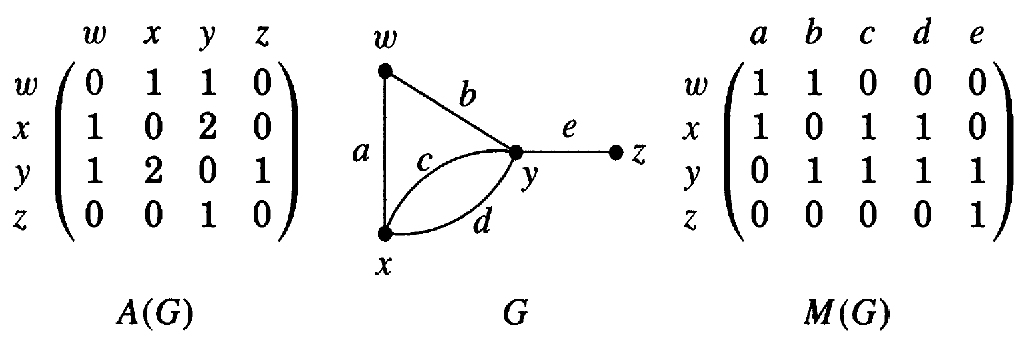
\includegraphics[width=.8\textwidth]{con-adj}
  \caption{A graph $G$ with its adjacency matrix $A(G)$ and incidence matrix $M(G)$. $a_{i,j}$ in $A(G)$ is $\set{v_i,\, v_j}$ in $G$.}
  \label{fig:con-adj}
\end{figure}

\begin{definition}{}{con-isomorphism}
  (1.1.20 Definition in text)
  An \textbf{isomorphism} from a \textbf{simple graph} $G$ to a \textbf{simple graph} $H$ is a \textbf{bijection function} (equivalent relation; \cref{def:intro-equiv-relation}) $\func{f}{V(G)}{V(H)}$ such that $uv \in E(G) \iff f(u)f(v) \in E(H)$. See \cref{def:con-loop} for the definition of simple graphs.

  We say "$G$ is \textbf{isomorphic to} $H$", written $G \cong H$, if there is an isomorphism from $G$ to $H$.
\end{definition}

You could recall three special function, including a bijective function as shown in \cref{fig:intro-special-functions}.
\reusefigure[ht]{fig:intro-special-functions}

For \cref{def:con-isomorphism}, in other words, a graph $G$ is isomorphic to a graph $H$ if and only if there exists a bijection function $\func{f}{V(G)}{V(H)}$, where $V(G)$ and $V(H)$ are vertices sets of $G$ and $H$ respectively, such that for every edge $uv$ in $G$, there is a corresponding edge $f(u)f(v)$ in $H$, and vice versa, without introducing additional vertices or edges.

For two isomorphic graphs $G$ and $H$, they may look different by human eyes. And note that a prerequisite for isomorphism is the same number of vertices and the same number of degrees. With different numbers of vertices or a degree that is absent one graph, the two graphs cannot be isomorphic. But with the same number of vertices and the same number of degrees, we still need a bijection function to prove the isomorphism from one graph to the other one.

See \cref{fig:con-isomorphism} for an example. In this example, we could see that vertices $w,\, z$ may correspond to $c,\, a$; and $x,\, y$ to $b,\, d$.

\supp{
  In programming, to determine whether graphs $G$ and $H$ are isomorphic to each other, we could build adjacency matrices for these two graphs (matrices 1 and 3 in \cref{fig:con-isomorphism}) respectively after fixing the order of vertices in $H$ to $a,\, b,\, c,\, d$ and choosing an order of vertices in $G$. Later, if the two adjacency matrices are different, change the order of vertices in $G$ to the other untested order, saying $w,\, y,\, z,\, x$, and then build the adjacency matrix of $G$ according to the new order. Note that for a new order of vertices, you cannot simply swap columns in the matrix because the row order changes as well. Once the adjacency matrices of $G$ and $H$ are identical like the matrices 2 and 2 in \cref{fig:con-isomorphism}, we could find the bijection function for vertex sets of $G$ and $H$. In \cref{fig:con-isomorphism}, vertices $w,\, y,\, z,\, x$ in $G$ correspond to vertices $a,\, b,\, c,\, d$ in $H$ respectively.

  The complexity of graph isomorphism is an open problem. It is highly possible not a $P$ problem. By the say, the subgraph problem (determining whether a smaller graph is isomorphic to some subgraph(s) in a larger graph) is NP-complete.

  A bonus problem (not in 2024 spring) is as follows. How do you define two multigraphs (including the cases of multiple edges and loops; see \cref{def:con-loop} for definition) are isomorphism? We need definition rather than proofs. Isomorphism in multigraphs is possible in real world. There is no commonly approved definition, but many different definitions you can reference. Note that graph (multigraph) isomorphism always follows the principle of bijection (one-to-one correspondence). Your answer has to be handwritten in Chinese clearly, possibly using the same ideas from references.
}

\begin{figure}[ht]
  \centering
  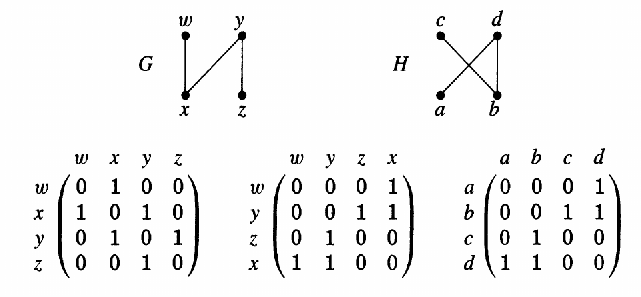
\includegraphics[width=.7\textwidth]{con-isomorphism}
  \caption{An example that $G$ is isomorphic to $H$. The following three matrices are adjacency matrices.}
  \label{fig:con-isomorphism}
\end{figure}

\subsection{Vertex Degrees and Counting}

\subsection{Directed Graphs}

\end{document}